\documentclass[11pt]{standalone}
\usepackage{amssymb}
\usepackage{amsmath}
\usepackage[no-math]{fontspec}
\usepackage{unicode-math}
\usepackage{libertinus}
\usepackage{pgf,xcolor}
\usepackage{tikz}
\usetikzlibrary{arrows.meta, backgrounds}
\usepackage{pgfplots}
\pgfplotsset{compat=newest}

\definecolor{my_darkgray}{HTML}{484949}
\definecolor{my_lightgray}{HTML}{F3F4F4}
\definecolor{my_darkblue}{HTML}{005A94}
\definecolor{my_lightblue}{HTML}{CCDEE9}
\definecolor{my_yellow}{HTML}{FFEC7F}
\definecolor{my_red}{HTML}{E60000}
\definecolor{my_orange}{HTML}{E87846}

\begin{document}
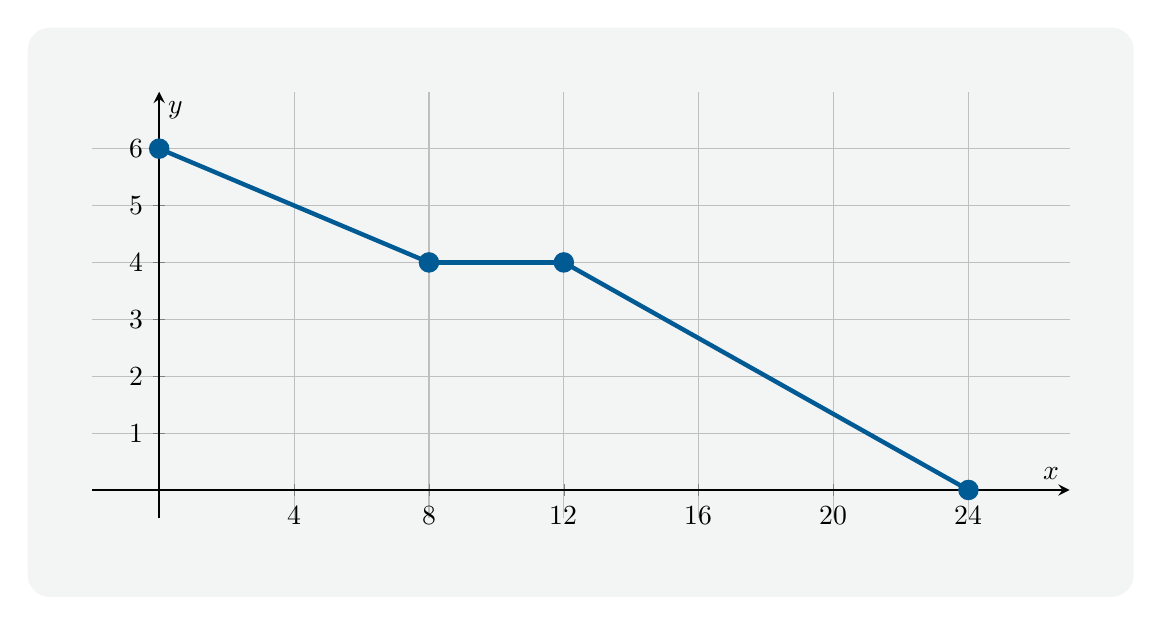
\begin{tikzpicture}[
    show background rectangle,
    background rectangle/.style={fill=my_lightgray, rounded corners=8pt},
    inner frame sep=0.8cm
]
\begin{axis}[
    axis lines = center,
    xlabel = {$x$},
    ylabel = {$y$},
    height=7cm, width=14cm,
    xmin=-2, xmax=27,
    ymin=-0.5, ymax=7,
    xtick={0,4,8,12,16,20,24},
    ytick={0,1,2,3,4,5,6},
    grid = both,
    axis line style={thick},
]

% Segment 1: h(x) = -0.25x + 6,  x in [0, 8]
\addplot[draw=my_darkblue, samples=200, ultra thick, domain=0:8]
    {-0.25*x + 6};

% Segment 2: h(x) = 4,  x in (8, 12]
\addplot[draw=my_darkblue, samples=200, ultra thick, domain=8:12]
    {4};

% Segment 3: h(x) = -x/3 + 8,  x in (12, 24]
\addplot[draw=my_darkblue, samples=200, ultra thick, domain=12:24]
    {-x/3 + 8};

% Filled circles at all four boundary points.
% The function is continuous at x=8 and x=12 (both segments meet at h=4),
% so a filled circle is sufficient at each junction.
% (0,  6): left endpoint,  included in segment 1 via [0,  8]
% (8,  4): right endpoint of segment 1, included via [0,  8]
%          left  endpoint of segment 2, excluded via (8, 12] -- same height
% (12, 4): right endpoint of segment 2, included via (8, 12]
%          left  endpoint of segment 3, excluded via (12,24] -- same height
% (24, 0): right endpoint of segment 3, included via (12,24]
\addplot[only marks, mark=*, mark size=3.5pt,
         draw=my_darkblue, fill=my_darkblue]
    coordinates {(0,6) (8,4) (12,4) (24,0)};

\end{axis}
\end{tikzpicture}
\end{document}
